\documentclass[12pt, a4paper]{article}
\usepackage{fullpage}
\usepackage{amsmath}
\usepackage{graphicx}
\usepackage{natbib}
\usepackage[version=3]{mhchem}
\usepackage{indentfirst}
%\usepackage{epstopdf}
%\usepackage{chemstyle}
\title{Add Hg Reactions from PHREEQC Database to PFLOTRAN Database}
\author{Guoping Tang}
\date\today{}

\begin{document}
\maketitle

\begin{abstract}
The Hg related reactions from PHREEQC database (phreeqc-scb.dat) are added into
PFLOTRAN database (hanford.dat). We conduct speciation calculations with the
cases in Dong et al. (2010) with PFLOTRAN and PHREEQC. The calculated results
are in general agreement, indicating the consistency of the two databases and
codes. Minor differences can be introduced when various activity calculation
options are used in PFLOTRAN. For competition for ligands among metals such as
Fe$^{3+}$, Cu$^{2+}$, as shown in Fig. 4 in Dong et al. (2010), differences in
the complexation reactions for these metals between the two databases may
introduce substantial differences in the calculation results.  
\end{abstract}

\section{Reactions}
\subsection{Hg$^{2+}$ Aqueous Complexation Reactions with Inorganic Species}

\begin{align}
%+'HgOH+' 3 1.0 'Hg++' 1.0 'H2O' -1.0 'H+' 500.000 3.3970 500.00 500.000 500.000 500.000 500.000 500.000 4.0 1.0 217.5973 'scb'
& \ce{Hg^2+ + H2O   <->  HgOH+ + H+} &&\mathrm{log\_k} = -3.397 \\
%+'Hg(OH)2' 3 1.0 'Hg++' 2.0 'H2O' -2.0 'H+' 500.000 5.980 500.00 500.000 500.000 500.000 500.000 500.000 4.0 0.0 234.6046 'scb'
& \ce{Hg^2+ + 2 H2O <->  Hg(OH)2 + 2H+}  &&\mathrm{log\_k} = -5.98 \\
%+'Hg(OH)3-' 3 1.0 'Hg++' 3.0 'H2O' -3.0 'H+' 500.000 21.091 500.00 500.000 500.000 500.000 500.000 500.000 4.0 -1.0 251.6119 'scb'
& \ce{Hg^2+ + 3 H2O  <->  Hg(OH)3^- + 3H+} &&\mathrm{log\_k} = -21.091 \\
%+'Hg2OH+++' 3 2.0 'Hg++' 1.0 'H2O' -1.0 'H+' 500.000 3.2970 500.00 500.000 500.000 500.000 500.000 500.000 4.0 3.0 418.1873 'scb'
& \ce{2Hg^2+ + H2O  <->  Hg_2OH^3+ + H+} && \mathrm{log\_k} = -3.297 \\
%+'Hg3(OH)3+++' 3 3.0 'Hg++' 3.0 'H2O' -3.0 'H+' 500.000 6.3910 500.00 500.000 500.000 500.000 500.000 500.000 4.0 3.0 652.7919 'scb'
& \ce{3Hg^2+ + 3H2O  <->  Hg_3(OH)_3^3+ + 3H+} && \mathrm{log\_k} = -6.391 \\
%+'HgBr+' 2 1.0 'Hg++' 1.0 'Br-' 500.000 -9.6100 500.000 500.000 500.000 500.000 500.000 500.000 4.0 1.0 280.494 'scb'
& \ce{Hg^2+ + Br^- <-> HgBr^+} && \mathrm{log\_k} = 9.61 \\
%+'HgBr2' 2 1.0 'Hg++' 2.0 'Br-' 500.000 -18.080 500.000 500.000 500.000 500.000 500.000 500.000 4.0 0.0 360.398 'scb'
& \ce{Hg^2+ + 2Br^- <-> HgBr2} && \mathrm{log\_k} = 18.08 \\
%+'HgBr3-' 2 1.0 'Hg++' 3.0 'Br-' 500.000 -20.510 500.000 500.000 500.000 500.000 500.000 500.000 4.0 -1.0 440.302 'scb'
& \ce{Hg^2+ + 3Br^- <-> HgBr_3^-} && \mathrm{log\_k} = 20.51 \\
%+'HgBr4--' 2 1.0 'Hg++' 4.0 'Br-' 500.000 -21.740 500.000 500.000 500.000 500.000 500.000 500.000 4.0 -2.0 520.206 'scb'
& \ce{Hg^2+ + 4Br^- <-> HgBr_4^2-} && \mathrm{log\_k} = 21.74 \\
%+'HgOHBr' 4 1.0 'Hg++' 1.0 'Br-' 1.0 'H2O' -1.0 'H+' 500.000 -6.2400 500.00 500.000 500.000 500.000 500.000 500.000 4.0 0.0 297.5013 'scb'
& \ce{Hg^2+ + Br^- + H2O <-> HgOHBr + H+} && \mathrm{log\_k} = 6.24 \\
%+'HgBrI' 3 1.0 'Hg++' 1.0 'Br-' 1.0 'I-' 500.000 -21.12 500.00 500.000 500.000 500.000 500.000 500.000 4.0 0.0 407.3985 'scb'
& \ce{Hg^2+ + Br^- + I- <-> HgBrI} && \mathrm{log\_k} = 21.12 \\
%+'HgBrI3--' 3 1.0 'Hg++' 1.0 'Br-' 3.0 'I-' 500.000 -28.020 500.00 500.000 500.000 500.000 500.000 500.000 4.0 -2.0 661.2075 'scb'
& \ce{Hg^2+ + Br^- + 3I- <-> HgBrI_3^2-} && \mathrm{log\_k} = 28.02 \\
%+'HgBr2I2--' 3 1.0 'Hg++' 2.0 'Br-' 2.0 'I-' 500.000 -26.800 500.00 500.000 500.000 500.000 500.000 500.000 4.0 -2.0 614.207 'scb'
& \ce{Hg^2+ + 2Br^- + 2I- <-> HgBr_2I_2^2-} && \mathrm{log\_k} = 26.80 \\
%+'HgCitrate-' 2 1.0 'Hg++' 1.0 'Citrate---' 500.000 -12.1900 500.00 500.000 500.000 500.000 500.000 500.000 4.0 -1.0 389.6913 'scb'
& \ce{Hg^2+ + Citrate^3- <-> HgCitrate-} && \mathrm{log\_k} = 12.19 \\
%+'HgCl+' 2 1.0 'Hg++' 1.0 'Cl-' -6.6100 -7.3100 -5.9000 -5.6500 -5.5000 -5.5000 -5.8000 -6.4000 4.0 1.0 236.0427 'scb+jin'
& \ce{Hg^2+ + Cl^- <-> HgCl^+} && \mathrm{log\_k} = 7.31 \\
%+'HgCl2' 2 1.0 'Hg++' 2.0 'Cl-' -14.160 -14.000 -12.250 -11.410 -10.710 -10.400 -10.300 -10.800 4.0 0.0 271.4954 'scb+jin'
& \ce{Hg^2+ + 2Cl^- <-> HgCl2} && \mathrm{log\_k} = 14.00 \\
%+'HgCl3-' 2 1.0 'Hg++' 3.0 'Cl-' -16.380 -14.925 -14.200 -13.250 -12.460 -12.100 -12.100 -12.700 4.0 -1.0 306.9481 'scb+jin'
& \ce{Hg^2+ + 3Cl^- <-> HgCl_3^-} && \mathrm{log\_k} = 14.925 \\
%+'HgCl4--' 2 1.0 'Hg++' 4.0 'Cl-' 500.000 -15.535 500.000 500.000 500.000 500.000 500.000 500.000 4.0 -2.0 342.4008 'scb'
& \ce{Hg^2+ + 4Cl^- <-> HgCl_4^2-} && \mathrm{log\_k} = 15.535 \\
%+'HgClI' 3 1.0 'Hg++' 1.0 'Cl-' 1.0 'I-' 500.000 -19.158 500.00 500.000 500.000 500.000 500.000 500.000 4.0 0.0 362.9472 'scb'
& \ce{Hg^2+ + Cl^- + I- <-> HgClI} && \mathrm{log\_k} = 19.158 \\
%+'HgOHCl' 4 1.0 'Hg++' 1.0 'Cl-' 1.0 'H2O' -1.0 'H+' 500.000 -4.2500 500.00 500.000 500.000 500.000 500.000 500.000 4.0 0.0 253.05 'scb'
& \ce{Hg^2+ + Cl^- + H2O <-> HgOHCl + H+} && \mathrm{log\_k} = 4.25 \\
%+'HgCO3' 2 1.0 'Hg++' 1.0 'CO3--' 500.000 -11.47 500.00 500.000 500.000 500.000 500.000 500.000 4.0 0.0 260.5992 'scb'
& \ce{Hg^2+ + CO3^2- <-> HgCO3} && \mathrm{log\_k} = 11.47 \\
%+'Hg(CO3)2--' 2 1.0 'Hg++' 2.0 'CO3--' 500.000 -15.042 500.00 500.000 500.000 500.000 500.000 500.000 4.0 -2.0 320.6084 'scb'
& \ce{Hg^2+ + 2 CO3^2- <-> Hg(CO3)_2^2-} && \mathrm{log\_k} = 15.042 \\
%+'HgHCO3+' 3 1.0 'Hg++' 1.0 'CO3--' 1.0 'H+' 500.000 -15.805 500.00 500.000 500.000 500.000 500.000 500.000 4.0 1.0 261.6071 'scb'
& \ce{Hg^2+ + HCO3^- <-> HgHCO3^+} && \mathrm{log\_k} = 15.805 \\
%+'HgOHCO3-' 4 1.0 'Hg++' 1.0 'CO3--' 1.0 'H2O' -1.0 'H+' 500.000 -5.33 500.00 500.000 500.000 500.000 500.000 500.000 4.0 1.0 277.6065 'scb'
& \ce{Hg^2+ + CO_3^2- + H2O <-> HgOHCO3^- + H+} && \mathrm{log\_k} = 5.33 \\
%+'HgEDTA--' 2 1.0 'Hg++' 1.0 'EDTA----' 500.000 -23.2200 500.00 500.000 500.000 500.000 500.000 500.000 4.0 -2.0 488.8034 'scb'
& \ce{Hg^2+ + EDTA^4- <-> HgEDTA^2-} && \mathrm{log\_k} = 23.22 \\
%+'HgHEDTA-' 3 1.0 'Hg++' 1.0 'EDTA----' 1.0 'H+' 500.000 -26.8500 500.00 500.000 500.000 500.000 500.000 500.000 4.0 -1.0 489.8113 'scb'
& \ce{Hg^2+ + EDTA^4- + H+ <-> HgHEDTA^-} && \mathrm{log\_k} = 26.85 \\
%+'HgH2EDTA' 3 1.0 'Hg++' 1.0 'EDTA----' 2.0 'H+' 500.000 -29.1500 500.00 500.000 500.000 500.000 500.000 500.000 4.0 0.0 490.8192 'scb'
& \ce{Hg^2+ + EDTA^4- + 2H+ <-> HgH2EDTA} && \mathrm{log\_k} = 29.15 \\
%+'HgOHEDTA---' 4 1.0 'Hg++' 1.0 'EDTA----' -1.0 'H+' 1.0 'H2O' 500.000 -13.6800 500.00 500.000 500.000 500.000 500.000 500.000 4.0 -3.0 505.8107 'scb'
& \ce{Hg^2+ + EDTA^4- + H2O <-> HgOHEDTA^3- + H+} && \mathrm{log\_k} = 13.68 \\
%+'HgF+' 2 1.0 'Hg++' 1.0 'F-'  500.000 -1.5700 500.000 500.000 500.000 500.000 500.000 500.000 4.0 1.0 219.5884 'scb'
& \ce{Hg^2+ + F^- <-> HgF^+} && \mathrm{log\_k} = 1.57
\end{align}
\begin{align}
%+'HgI+' 2 1.0 'Hg++' 1.0 'I-' 500.000 -13.410 500.000 500.000 500.000 500.000 500.000 500.000 4.0 1.0 327.4945 'scb'
& \ce{Hg^2+ + I^- <-> HgI^+} && \mathrm{log\_k} = 13.41 \\
%+'HgI2' 2 1.0 'Hg++' 2.0 'I-' 500.000 -24.630 500.000 500.000 500.000 500.000 500.000 500.000 4.0 0.0 454.399 'scb'
& \ce{Hg^2+ + 2I^- <-> HgI2} && \mathrm{log\_k} = 24.63 \\
%+'HgI3-' 2 1.0 'Hg++' 3.0 'I-' 500.000 -28.410 500.000 500.000 500.000 500.000 500.000 500.000 4.0 -1.0 581.3035 'scb'
& \ce{Hg^2+ + 3I^- <-> HgI_3^-} && \mathrm{log\_k} = 28.41 \\
%+'HgI4--' 2 1.0 'Hg++' 4.0 'I-' 500.000 -30.340 500.000 500.000 500.000 500.000 500.000 500.000 4.0 -2.0 708.208 'scb'
& \ce{Hg^2+ + 4I^- <-> HgI_4^2-} && \mathrm{log\_k} = 30.34 \\
%+'HgOHI' 4 1.0 'Hg++' 1.0 'I-' 1.0 'H2O' -1.0 'H+' 500.000 -9.4100 500.00 500.000 500.000 500.000 500.000 500.000 4.0 0.0 344.5018 'scb'
& \ce{Hg^2+ + I^- + H2O <-> HgOHI + H+} && \mathrm{log\_k} = 9.41 \\
%+'HgNH3++' 3 1.0 'Hg++' 1.0 'NH4+' -1.0 'H+' 500.000 0.444 500.000 500.000 500.000 500.000 500.000 500.000 4.0 2.0 217.6206 'scb'
& \ce{Hg^2+ + NH4^+ <-> HgNH3^2+ + H+} && \mathrm{log\_k} = -0.444 \\
%+'Hg(NH3)2++' 3 1.0 'Hg++' 2.0 'NH4+' -2.0 'H+' 500.000 0.688 500.000 500.000 500.000 500.000 500.000 500.000 4.0 2.0 234.6512 'scb'
& \ce{Hg^2+ + 2 NH4^+ <-> Hg(NH3)2^2+ + 2H+} && \mathrm{log\_k} = -0.688 \\
%+'Hg(NH3)3++' 3 1.0 'Hg++' 3.0 'NH4+' -3.0 'H+' 500.000 9.432 500.000 500.000 500.000 500.000 500.000 500.000 4.0 2.0 251.6818 'scb'
& \ce{Hg^2+ + 3 NH4^+ <-> Hg(NH3)3^2+ + 3H+} && \mathrm{log\_k} = -9.432 \\
%+'Hg(NH3)4++' 3 1.0 'Hg++' 4.0 'NH4+' -4.0 'H+' 500.000 17.676 500.000 500.000 500.000 500.000 500.000 500.000 4.0 2.0 268.7124 'scb'
& \ce{Hg^2+ + 4 NH4^+ <-> Hg(NH3)4^2+ + 4H+} && \mathrm{log\_k} = -17.676 \\
%+'HgNO3+' 2 1.0 'Hg++' 1.0 'NO3-' 500.000 0.430 500.000 500.000 500.000 500.000 500.000 500.000 4.0 1.0 262.5949 'scb'
& \ce{Hg^2+ + NO_3^- <-> HgNO_3^+} && \mathrm{log\_k} = -0.43 \\
%+'Hg(NO3)2' 2 1.0 'Hg++' 2.0 'NO3-' 500.000 0.810 500.000 500.000 500.000 500.000 500.000 500.000 4.0 0.0 324.5998 'scb'
& \ce{Hg^2+ + 2 NO_3^- <-> Hg(NO_3)_2} && \mathrm{log\_k} = -0.81 \\
%+'HgPO4-' 2 1.0 'Hg++' 1.0 'PO4---' 500.000 -7.841 500.000 500.000 500.000 500.000 500.000 500.000 4.0 -1.0 295.5614 'scb'
& \ce{Hg^2+ + PO_4^3- <-> HgPO_4^-} && \mathrm{log\_k} = 7.841 \\
%+'HgHPO4' 3 1.0 'Hg++' 1.0 'PO4---' 1.0 'H+' 500.000 -20.056 500.000 500.000 500.000 500.000 500.000 500.000 4.0 0.0 296.5693 'scb'
& \ce{Hg^2+ + PO_4^3- + H+ <-> HgHPO_4} && \mathrm{log\_k} = 20.056 \\
%+'HgS' 3 1.0 'Hg++' 1.0 'HS-' -1.0 'H+' 500.000 -28.6 500.00 500.000 500.000 500.000 500.000 500.000 4.0 0.0 232.654 'scb'
& \ce{Hg^2+ + HS^- <-> HgS + H^+} && \mathrm{log\_k} = 28.6 \\
%+'HgS2--' 3 1.0 'Hg++' 2.0 'HS-' -2.0 'H+' 500.000 -24.73 500.00 500.000 500.000 500.000 500.000 500.000 4.0 -2.0 264.718 'scb'
& \ce{Hg^2+ + 2HS^- <-> HgS_2^2- + 2 H^+} && \mathrm{log\_k} = 24.73 \\
%+'Hg(HS)2' 2 1.0 'Hg++' 2.0 'HS-' 500.0 -39.77 500.00 500.000 500.000 500.000 500.000 500.000 4.0 0.0 266.7338 'scb'
& \ce{Hg^2+ + 2HS^- <-> Hg(S_2)_2} && \mathrm{log\_k} = 39.77 \\
%+'HgHS2-' 3 1.0 'Hg++' 2.0 'HS-' -1.0 'H+' 500.0 -33.44 500.00 500.000 500.000 500.000 500.000 500.000 4.0 -1.0 265.7259 'scb'
& \ce{Hg^2+ + 2HS^- <-> HgHS_2^- + H+} && \mathrm{log\_k} = 39.77 \\
%+'HgHS+' 2 1.0 'Hg++' 1.0 'HS-' 500.0 -20.5 500.00 500.000 500.000 500.000 500.000 500.000 4.0 1.0 233.6619 'scb'
& \ce{Hg^2+ + HS^- <-> HgHS^+} && \mathrm{log\_k} = 20.5 \\
%+'HgS5' 5 1.0 'Hg++' 5.0 'HS-' 3.0 'H+' -4.0 'H2O' 2.0 'O2' 500.000 -194.56 500.00 500.000 500.000 500.000 500.000 500.000 4.0 0.0 360.91 'scb'
& \ce{Hg^2+ + 5 HS^- + 3 H^+ 2 O_2 <-> HgS_5 + 4 H2O} && \mathrm{log\_k} = 194.56 \\
%+'Hg(S5)2--' 5 1.0 'Hg++' 10.0 'HS-' 6.0 'H+' -8.0 'H2O' 4.0 'O2' 500.000 -352.0 500.00 500.000 500.000 500.000 500.000 500.000 4.0 -2.0 521.23 'scb'
& \ce{Hg^2+ + 10 HS^- + 6 H^+ 4 O_2 <-> Hg(S_5)_2^2- + 8 H2O} && \mathrm{log\_k} = 352.0 \\
%+'HgS5OH-' 5 1.0 'Hg++' 5.0 'HS-' 2.0 'H+' -3.0 'H2O' 2.0 'O2' 500.000 -185.98 500.00 500.000 500.000 500.000 500.000 500.000 4.0 -1.0 377.9173 'scb'
& \ce{Hg^2+ + 5 HS^- + 2 H^+ 2 O_2 <-> HgS_5OH^- + 3 H2O} && \mathrm{log\_k} = 185.98 \\
%+'Hg(S2O3)2--' 2 1.0 'Hg++' 2.0 'S2O3--' 500.000 -29.48 500.00 500.000 500.000 500.000 500.000 500.000 4.0 -2.0 424.8504 'scb'
& \ce{Hg^2+ + 2 S_2O_3^2- <-> Hg(S2O3)_2^2-} && \mathrm{log\_k} = 29.48 \\
%+'Hg(S2O3)3---' 2 1.0 'Hg++' 3.0 'S2O3--' 500.000 -31.28 500.00 500.000 500.000 500.000 500.000 500.000 4.0 -3.0 536.9806 'scb'
& \ce{Hg^2+ + 3 S_2O_3^2- <-> Hg(S2O3)_3^3-} && \mathrm{log\_k} = 31.28 \\
%+'HgSO4' 2 1.0 'Hg++' 1.0 'SO4--' 500.0 -2.42 500.0 500.0 500.0 500.0 500.0 500.0 4.0 0.0 296.6536 'scb'
& \ce{Hg^2+ + SO_4^2- <-> HgSO4} && \mathrm{log\_k} = 2.42 \\
%+'Hg(SO4)2--' 2 1.0 'Hg++' 2.0 'SO4--' 500.0 -3.48 500.0 500.0 500.0 500.0 500.0 500.0 4.0 -2.0 392.7172 'scb'
& \ce{Hg^2+ + 2 SO_4^2- <-> Hg(SO4)_2^2-} && \mathrm{log\_k} = 3.48
\end{align}

\subsection{CH$_4$Hg$^{+}$ Aqueous Complexation Reactions with Inorganic Species}
\begin{align}
%+'MmmOH' 3 1.0 'Mmm+' 1.0 'H2O' -1.0 'H+' 500.0 4.557 500.0 500.0 500.0 500.0 500.0 500.0 4.0 0.0 232.6323
& \ce{CH3Hg+ + H2O <-> CH3HgOH + H+} && \mathrm{log\_k} =  -4.557 \\
%+'(Mmm)2OH+' 3 2.0 'Mmm+' 1.0 'H2O' -1.0 'H+' 500.0 1.997 500.0 500.0 500.0 500.0 500.0 500.0 4.0 1.0 448.2573
& \ce{2 CH3Hg+ + H2O <-> (CH3Hg)2OH^+ + H+} && \mathrm{log\_k} =  -1.997 \\
%+'MmmCO3-' 2 1.0 'Mmm+' 1.0 'CO3--' 500.0 -6.511 500.0 500.0 500.0 500.0 500.0 500.0 4.0 -1.0 275.6342
& \ce{CH3Hg+ + CO_3^2- <-> CH3HgCO_3^-} && \mathrm{log\_k} =  6.511 \\
%+'MmmNH3+' 3 1.0 'Mmm+' 1.0 'NH4+' -1.0 'H+' 500.0 1.644 500.0 500.0 500.0 500.0 500.0 500.0 4.0 1.0 232.6556
& \ce{CH3Hg+ + NH_4^+ <-> CH3HgNH_3^+ + H^+} && \mathrm{log\_k} =  -1.644 \\
%+'MmmHPO4-' 3 1.0 'Mmm+' 1.0 'PO4---' 1.0 'H+' 500.0 -17.806 500.0 500.0 500.0 500.0 500.0 500.0 4.0 -1.0 311.6043
& \ce{CH3Hg+ PO_4^3- + H^+ <-> CH3HgHPO_4^-} && \mathrm{log\_k} =  17.806 \\
%+'MmmSO4-' 2 1.0 'Mmm+' 1.0 'SO4--' 500.0 -2.0 500.0 500.0 500.0 500.0 500.0 500.0 4.0 -1.0 311.6886
& \ce{CH3Hg+ + SO_4^2- <-> CH3HgSO_4^-} && \mathrm{log\_k} =  2.0 \\
%+'MmmS-' 3 1.0 'Mmm+' 1.0 'HS-' -1.0 'H+' 500.0 -7.0 500.0 500.0 500.0 500.0 500.0 500.0 4.0 -1.0 247.689
& \ce{CH3Hg+ + HS- <-> CH3HgS^- + H^+} && \mathrm{log\_k} =  7.0 \\
%+'Mmm2S' 3 2.0 'Mmm+' 1.0 'HS-' -1.0 'H+' 500.0 -23.51 500.0 500.0 500.0 500.0 500.0 500.0 4.0 0.0 463.314
& \ce{2 CH3Hg+ + HS- <-> (CH3Hg)_2S + H^+} && \mathrm{log\_k} =  23.51 \\
%+'Mmm3S+' 3 3.0 'Mmm+' 1.0 'HS-' -1.0 'H+' 500.0 -30.51 500.0 500.0 500.0 500.0 500.0 500.0 4.0 1.0 678.939
& \ce{3 CH3Hg+ + HS- <-> (CH3Hg)_3S^+ + H^+} && \mathrm{log\_k} =  30.51 \\
%+'MmmF' 2 1.0 'Mmm+' 1.0 'F-' 500.0 -1.71 500.0 500.0 500.0 500.0 500.0 500.0 4.0 0.0 234.6234
& \ce{CH3Hg+ + F- <-> CH3HgF} && \mathrm{log\_k} =  1.71 \\
%+'MmmCl' 2 1.0 'Mmm+' 1.0 'Cl-' 500.0 -5.39 500.0 500.0 500.0 500.0 500.0 500.0 4.0 0.0 251.0777
& \ce{CH3Hg+ + Cl- <-> CH3HgCl} && \mathrm{log\_k} =  5.39 \\
%+'MmmBr' 2 1.0 'Mmm+' 1.0 'Br-' 500.0 -6.7 500.0 500.0 500.0 500.0 500.0 500.0 4.0 0.0 295.529
& \ce{CH3Hg+ + Br- <-> CH3HgBr} && \mathrm{log\_k} =  6.7 \\
%+'MmmI' 2 1.0 'Mmm+' 1.0 'I-' 500.0 -8.71 500.0 500.0 500.0 500.0 500.0 500.0 4.0 0.0 342.5295
& \ce{CH3Hg+ + I- <-> CH3HgI} && \mathrm{log\_k} =  8.71 \\
%+'MmmI2-' 2 1.0 'Mmm+' 2.0 'I-' 500.0 -9.18 500.0 500.0 500.0 500.0 500.0 500.0 4.0 -1.0 469.434
& \ce{CH3Hg+ + 2 I- <-> CH3HgI_2^-} && \mathrm{log\_k} =  9.18 \\
%+'MmmS2O3-' 2 1.0 'Mmm+' 1.0 'S2O3--' 500.0 -11.18 500.0 500.0 500.0 500.0 500.0 500.0 4.0 -1.0 327.7512
& \ce{CH3Hg+ + S_2O3^2- <-> CH3HgS_2O_3^-} && \mathrm{log\_k} =  11.18
\end{align}

\subsection{Hg$^{2+}$ and CH$_4$Hg$^{+}$ Aqueous Complexation Reactions with Organic Species}

\begin{align}
%+'HDom---' 2 1.0 'H+' 1.0 'Dom----' 500.0 -10.0 500.0 500.0 500.0 500.0 500.0 500.0 4.0 -3.0 12.0111 'scb'
& \ce{H+ + DOM^4- <-> HDom^3-} && \mathrm{log\_k} = 10.0 \\
%'HgDom--' 2 1.0 'Hg++' 1.0 'Dom----' 500.0 -21.4 500.0 500.0 500.0 500.0 500.0 500.0 4.0 -2.0 212.6011 'scb'
& \ce{Hg^2+ + DOM^4- <-> HgDom^2-} && \mathrm{log\_k} = 21.4 \\
%+'RcooH' 2 1.0 'Rcoo-' 1.0 'H+' 500.0 -4.5 500.0 500.0 500.0 500.0 500.0 500.0 4.0 0.0 13.019 'scb'
& \ce{H+ + Rcoo^- <-> RcooH} && \mathrm{log\_k} = 4.5 \\
%+'HgRcoo+' 2 1.0 'Hg++' 1.0 'Rcoo-' 500.0 -10.0 500.0 500.0 500.0 500.0 500.0 500.0 4.0 1.0 212.6011 'scb'
& \ce{Hg^2+ + Rcoo^- <-> HgRcoo^+} && \mathrm{log\_k} = 10.0 \\
%+'RsH' 2 1.0 'Rs-' 1.0 'H+' 500.0 -10.0 500.0 500.0 500.0 500.0 500.0 500.0 4.0 0.0 33.0719 'scb'
& \ce{H+ + Rs^- <-> RsH} && \mathrm{log\_k} = 10.0 \\
%+'HgRs+' 2 1.0 'Hg++' 1.0 'Rs-' 500.0 -21.0 500.0 500.0 500.0 500.0 500.0 500.0 4.0 1.0 232.654 'scb'
& \ce{Hg^2+ + Rs^- <-> HgRs^+} && \mathrm{log\_k} = 21.0 \\
%+'HgRs2' 2 1.0 'Hg++' 2.0 'Rs-' 500.0 -28.7 500.0 500.0 500.0 500.0 500.0 500.0 4.0 0.0 264.718 'scb'
& \ce{Hg^2+ + 2 Rs^- <-> HgRs_2} && \mathrm{log\_k} = 28.7 \\
%+'MmmRs' 2 1.0 'Mmm+' 1.0 'Rs-' 500.0 -14.0 500.0 500.0 500.0 500.0 500.0 500.0 4.0 0.0 247.689 'scb'
& \ce{CH_3Hg+ + Rs^- <-> CH_3HgRs} && \mathrm{log\_k} = 14.0 \\
%+'HL' 2 1.0 'H+' 1.0 'L-' 500.0 -10.0 500.0 500.0 500.0 500.0 500.0 500.0 4.0 0.0 13.019 'scb'
& \ce{H+ + L^- <-> HL} && \mathrm{log\_k} = 10.0 \\
%+'HgL+' 2 1.0 'Hg++' 1.0 'L-' 500.0 -21.27 500.0 500.0 500.0 500.0 500.0 500.0 4.0 1.0 212.6011 'scb'
& \ce{Hg^2+ + L^- <-> HgL^+} && \mathrm{log\_k} = 21.27 \\
%+'HgL2' 2 1.0 'Hg++' 2.0 'L-' 500.0 -34.04 500.0 500.0 500.0 500.0 500.0 500.0 4.0 0.0 224.6122 'scb'
& \ce{Hg^2+ + 2 L^- <-> HgL_2} && \mathrm{log\_k} = 34.04 \\
%+'MmmL' 2 1.0 'Mmm+' 1.0 'L-' 500.0 -16.76 500.0 500.0 500.0 500.0 500.0 500.0 4.0 0.0 227.6361 'scb'
& \ce{CH_3Hg^+ + L^- <-> CH_3HgL} && \mathrm{log\_k} = 16.76 \\
%+'CaL+' 2 1.0 'Ca++' 1.0 'L-' 500.0   -4.3 500.0 500.0 500.0 500.0 500.0 500.0 4.0 1.0  52.0891 'scb'
& \ce{Ca^2+ + L^- <-> CaL^+} && \mathrm{log\_k} = 4.3 \\
%+'MgL+' 2 1.0 'Mg++' 1.0 'L-' 500.0  -3.61 500.0 500.0 500.0 500.0 500.0 500.0 4.0 1.0  36.3161 'scb'
& \ce{Mg^2+ + L^- <-> MgL^+} && \mathrm{log\_k} = 3.61 \\
%+'ZnL+' 2 1.0 'Zn++' 1.0 'L-' 500.0  -9.69 500.0 500.0 500.0 500.0 500.0 500.0 4.0 1.0  77.4011 'scb'
& \ce{Zn^2+ + L^- <-> ZnL^+} && \mathrm{log\_k} = 9.69 \\
%+'ZnL2' 2 1.0 'Zn++' 2.0 'L-' 500.0 -16.10 500.0 500.0 500.0 500.0 500.0 500.0 4.0 0.0  89.4122 'scb'
& \ce{Zn^2+ + 2 L^- <-> ZnL_2} && \mathrm{log\_k} = 16.10 \\
%+'CuL+' 2 1.0 'Cu++' 1.0 'L-' 500.0  -12.0 500.0 500.0 500.0 500.0 500.0 500.0 4.0 1.0  75.5571 'scb'
& \ce{Cu^2+ + L^- <-> CuL^+} && \mathrm{log\_k} = 12.0 \\
%+'CuL2' 2 1.0 'Cu++' 2.0 'L-' 500.0 -16.95 500.0 500.0 500.0 500.0 500.0 500.0 4.0 0.0  87.5682 'scb'
& \ce{Cu^2+ + 2 L^- <-> CuL_2} && \mathrm{log\_k} = 16.95 \\
%+'NiL+' 2 1.0 'Ni++' 1.0 'L-' 500.0  -9.72 500.0 500.0 500.0 500.0 500.0 500.0 4.0 1.0  70.7011 'scb'
& \ce{Ni^2+ + L^- <-> NiL^+} && \mathrm{log\_k} = 9.72 \\
%+'NiL2' 2 1.0 'Ni++' 2.0 'L-' 500.0 -15.96 500.0 500.0 500.0 500.0 500.0 500.0 4.0 0.0  82.7122 'scb'
& \ce{Ni^2+ + 2 L^- <-> NiL_2} && \mathrm{log\_k} = 15.96 \\
%+'CdL+' 2 1.0 'Cd++' 1.0 'L-' 500.0 -10.62 500.0 500.0 500.0 500.0 500.0 500.0 4.0 1.0 124.4221 'scb'
& \ce{Cd^2+ + L^- <-> CdL^+} && \mathrm{log\_k} = 10.62 \\
%+'CdL2' 2 1.0 'Cd++' 2.0 'L-' 500.0 -17.48 500.0 500.0 500.0 500.0 500.0 500.0 4.0 0.0 136.4332 'scb'
& \ce{Cd^2+ + 2 L^- <-> CdL_2} && \mathrm{log\_k} = 17.48 \\
%+'PbL+' 2 1.0 'Pb++' 1.0 'L-' 500.0 -11.83 500.0 500.0 500.0 500.0 500.0 500.0 4.0 1.0 219.2111 'scb'
& \ce{Pb^2+ + L^- <-> PbL^+} && \mathrm{log\_k} = 11.83 \\
%+'PbL2' 2 1.0 'Pb++' 2.0 'L-' 500.0 -15.86 500.0 500.0 500.0 500.0 500.0 500.0 4.0 0.0 231.2222 'scb'
& \ce{Pb^2+ + 2 L^- <-> PbL_2} && \mathrm{log\_k} = 15.86 \\
%+'CoL+' 2 1.0 'Co++' 1.0 'L-' 500.0 -10.62 500.0 500.0 500.0 500.0 500.0 500.0 4.0 1.0  70.9443 'scb'
& \ce{Co^2+ + L^- <-> CoL^+} && \mathrm{log\_k} = 10.62 \\
%+'CoL2' 2 1.0 'Co++' 2.0 'L-' 500.0 -17.48 500.0 500.0 500.0 500.0 500.0 500.0 4.0 0.0  82.9554 'scb'
& \ce{Co^2+ + 2 L^- <-> CoL_2} && \mathrm{log\_k} = 17.48 \\
%+'UO2L2' 2 1.0 'UO2++' 2.0 'L-' 500.0 -10.19 500.0 500.0 500.0 500.0 500.0 500.0 4.0 0.0 294.0499 'scb'
& \ce{UO_2^2+ + 2 L^- <-> UO_2L_2} && \mathrm{log\_k} = 10.19 \\
%+'FeL++' 2 1.0 'Fe+++' 1.0 'L-' 500.0 -12.28 500.0 500.0 500.0 500.0 500.0 500.0 4.0 2.0  67.8581 'scb'
& \ce{Fe^3+ + L^- <-> FeL^2+} && \mathrm{log\_k} = 12.28 \\
%+'FeL2+' 2 1.0 'Fe+++' 2.0 'L-' 500.0 -16.40 500.0 500.0 500.0 500.0 500.0 500.0 4.0 1.0  79.8692 'scb'
& \ce{Fe^3+ + 2 L^- <-> FeL_2^+} && \mathrm{log\_k} = 16.40
\end{align}

\subsection{Other Metals}
%+'Cu(OH)2' 3 -2.0000 'H+' 1.0000 'Cu++' 2.0000 'H2O' 500.0000 13.68 500.0000 500.0000 500.0000 500.0000 500.0000 500.0000 4.0 1.0 97.5606 'scb' 

\section{Example Calculations}


\emph{Example 1. Sulfate reduction with acetate as the electron donor}
\\
\begin{figure}[h]
\centering
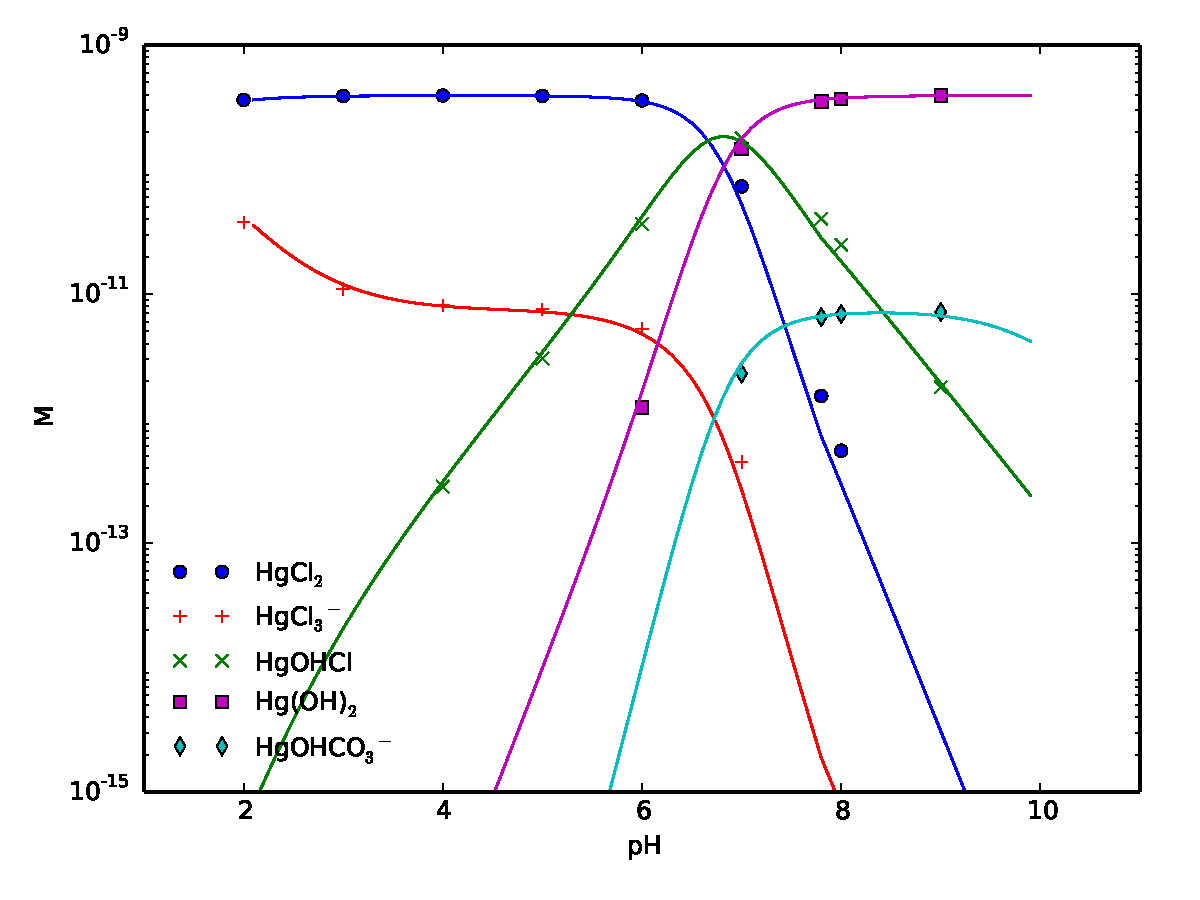
\includegraphics[width=0.5\textwidth]{../pflotran/speciation/Dong2010/ex1/comp.pdf}
\caption{xxx}
\label{Fig1}
\end{figure}

\emph{Example 2. Sulfate reduction with acetate as the electron donor and with nitrate inhibition}
\\
\begin{figure}[h]
\centering
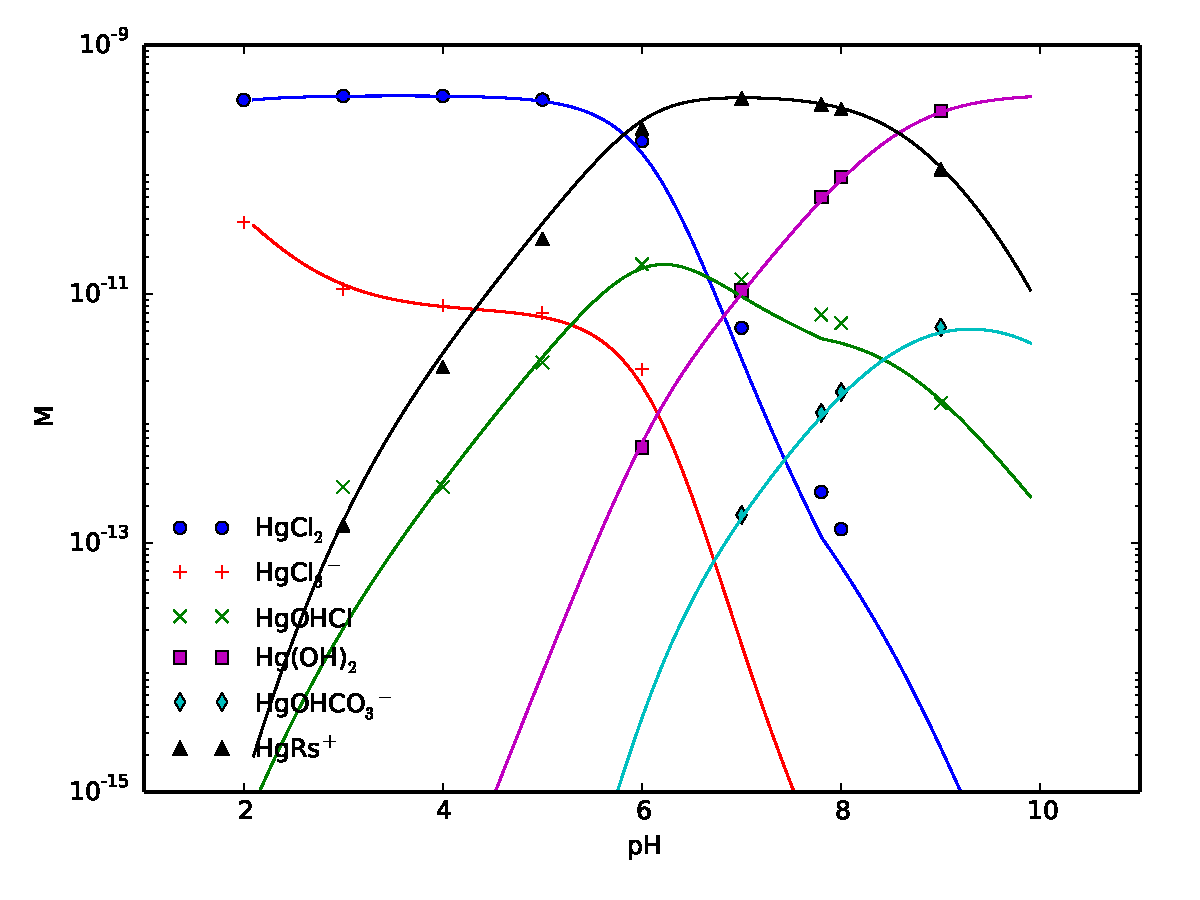
\includegraphics[width=0.5\textwidth]{../pflotran/speciation/Dong2010/ex2/ex2.pdf}
\caption{xxx}
\label{Fig2}
\end{figure}

\emph{Example 3. Sulfate reduction with acetate as the electron donor and with nitrate inhibition}
\\
\begin{figure}[h]
\centering
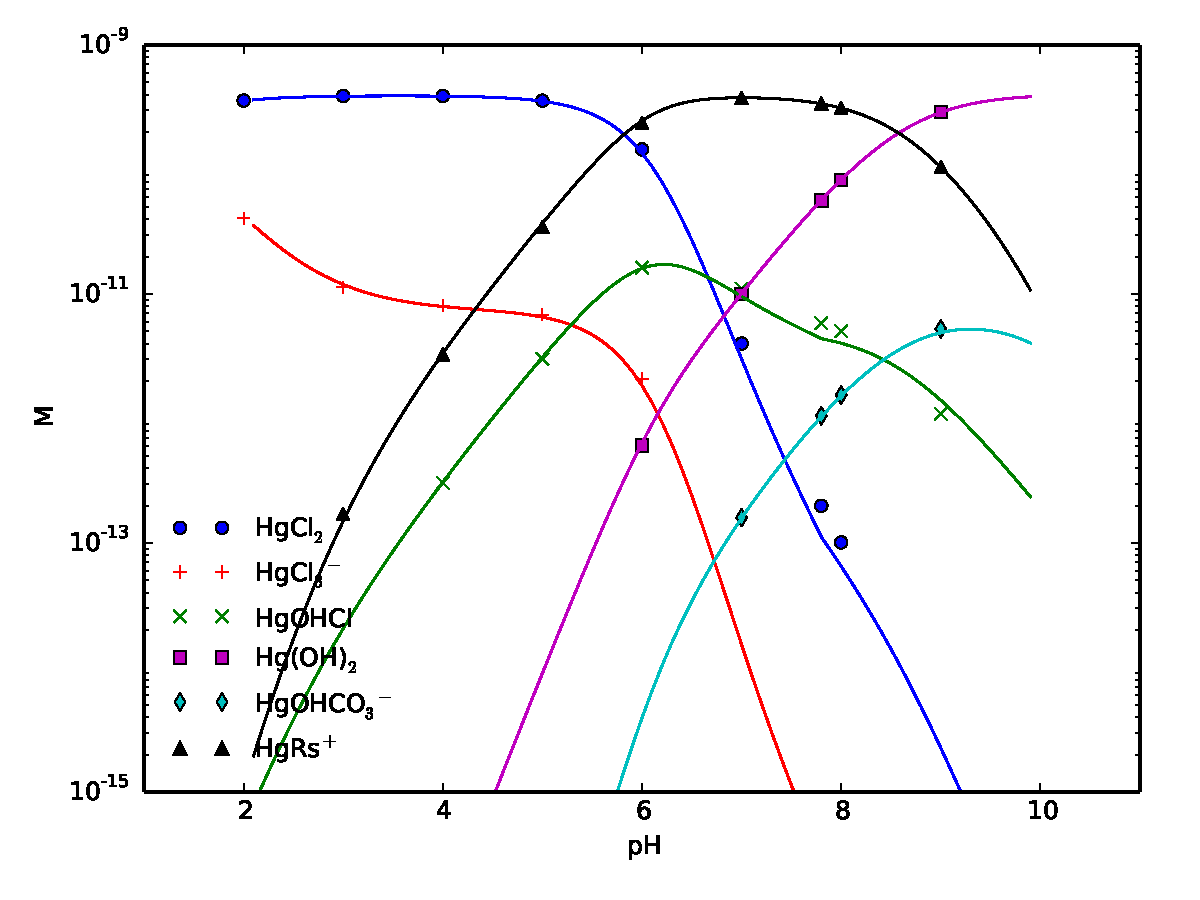
\includegraphics[width=0.5\textwidth]{../pflotran/speciation/Dong2010/ex2a/ex2.pdf}
\caption{xxx}
\label{Fig2a}
\end{figure}

\emph{Example 4. Sulfate reduction with acetate as the electron donor and with nitrate inhibition}
\\
\begin{figure}[h]
\centering
\includegraphics[width=0.5\textwidth]{../pflotran/speciation/Dong2010/ex3/ex3.pdf}
\caption{xxx}
\label{Fig3}
\end{figure}

\emph{Example 5. Sulfate reduction with acetate as the electron donor and with nitrate inhibition}
\\
\begin{figure}[h]
\centering
\includegraphics[width=0.5\textwidth]{../pflotran/speciation/Dong2010/ex3/ex3.pdf}
\caption{xxx}
\label{Fig3}
\end{figure}

\emph{Example 6. Sulfate reduction with acetate as the electron donor and with nitrate inhibition}
\\
\begin{figure}[h]
\centering
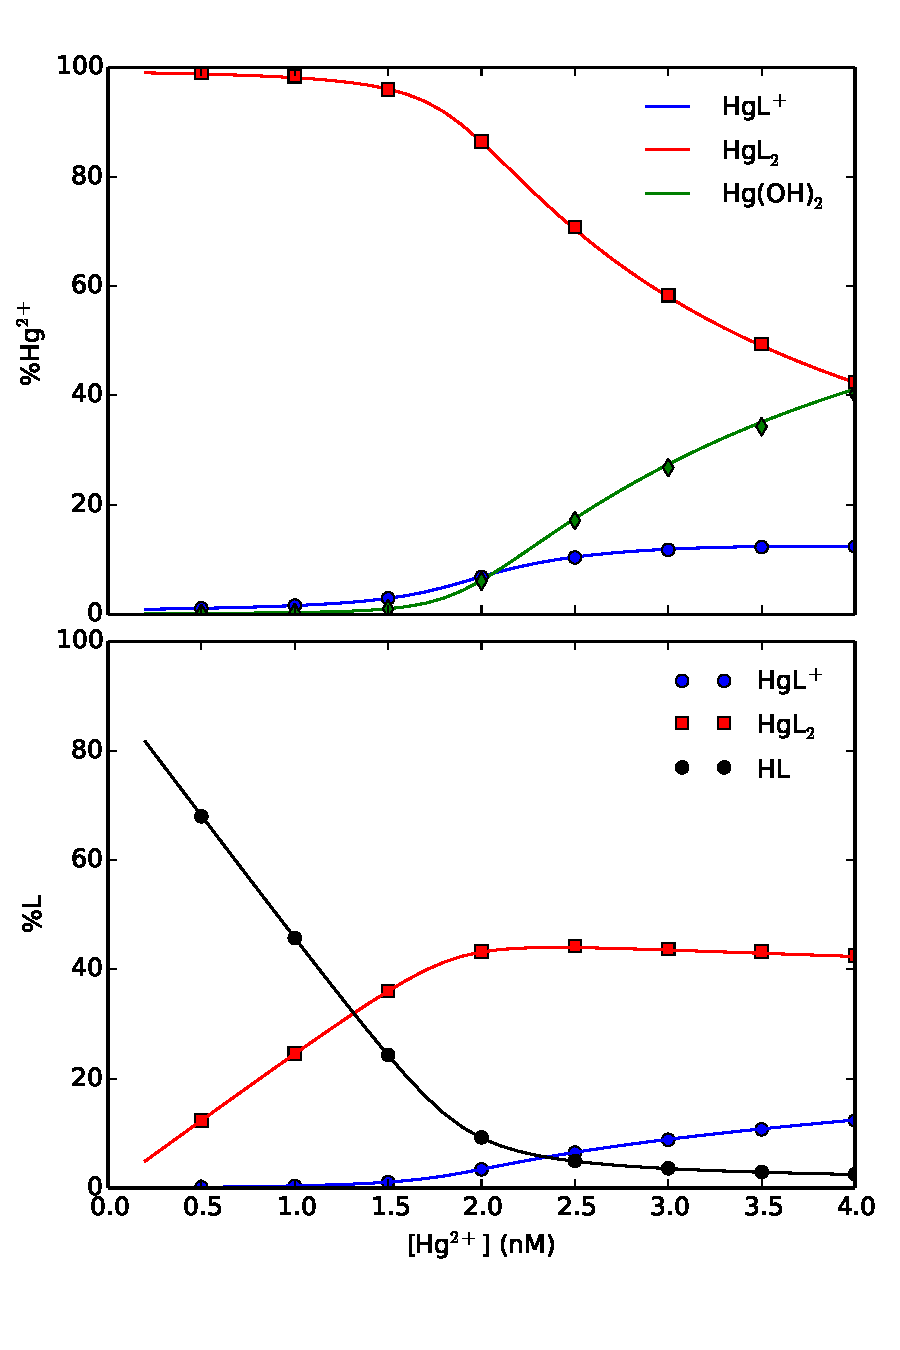
\includegraphics[width=0.5\textwidth]{../pflotran/speciation/Dong2010/ex4/ex40.pdf}
\caption{xxx}
\label{Fig40}
\end{figure}

\\
\begin{figure}[h]
\centering
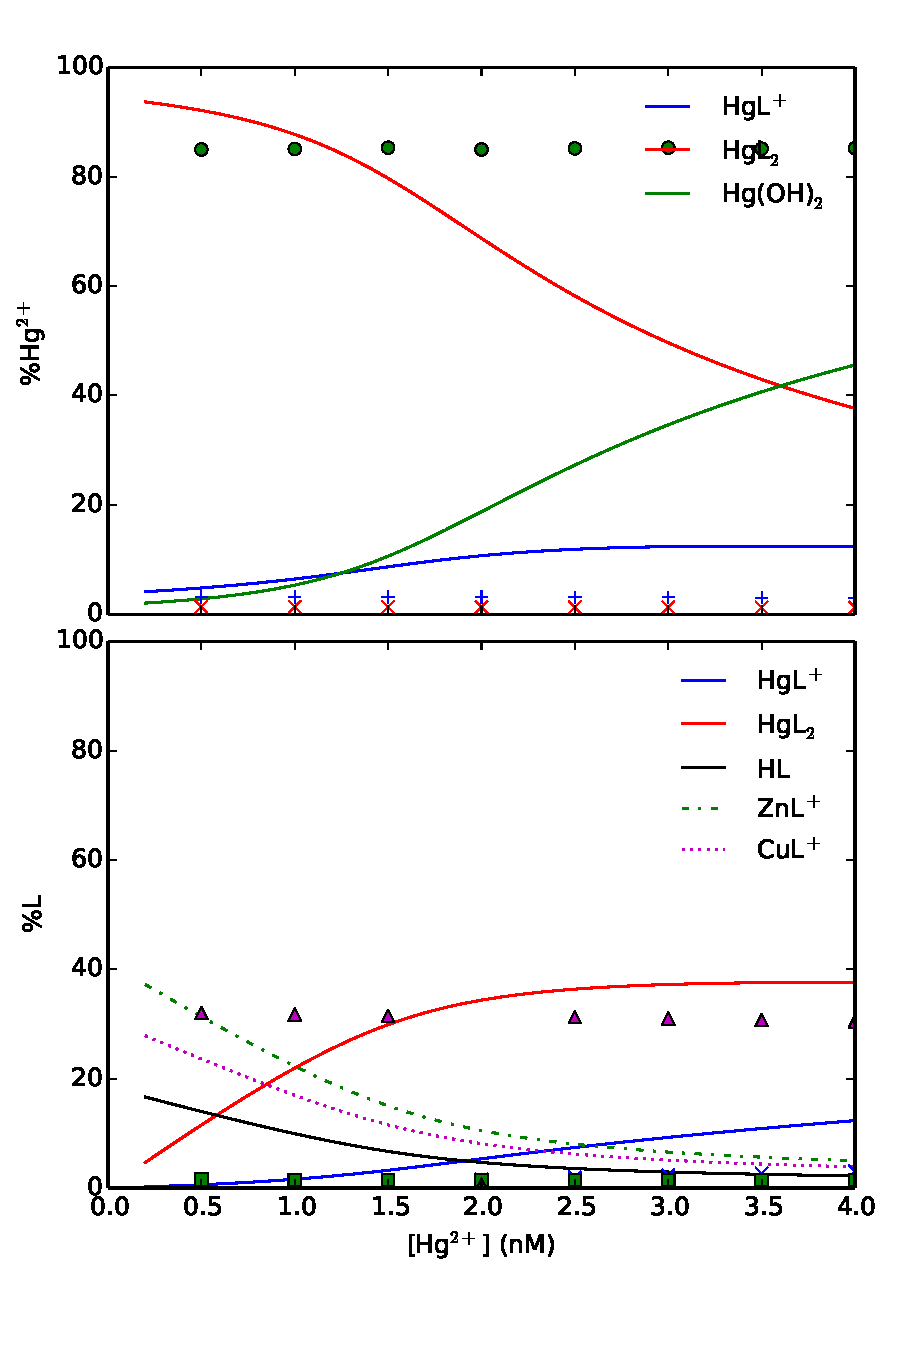
\includegraphics[width=0.5\textwidth]{../pflotran/speciation/Dong2010/ex4/ex4a.pdf}
\caption{xxx}
\label{Fig4a}
\end{figure}

\\
\begin{figure}[h]
\centering
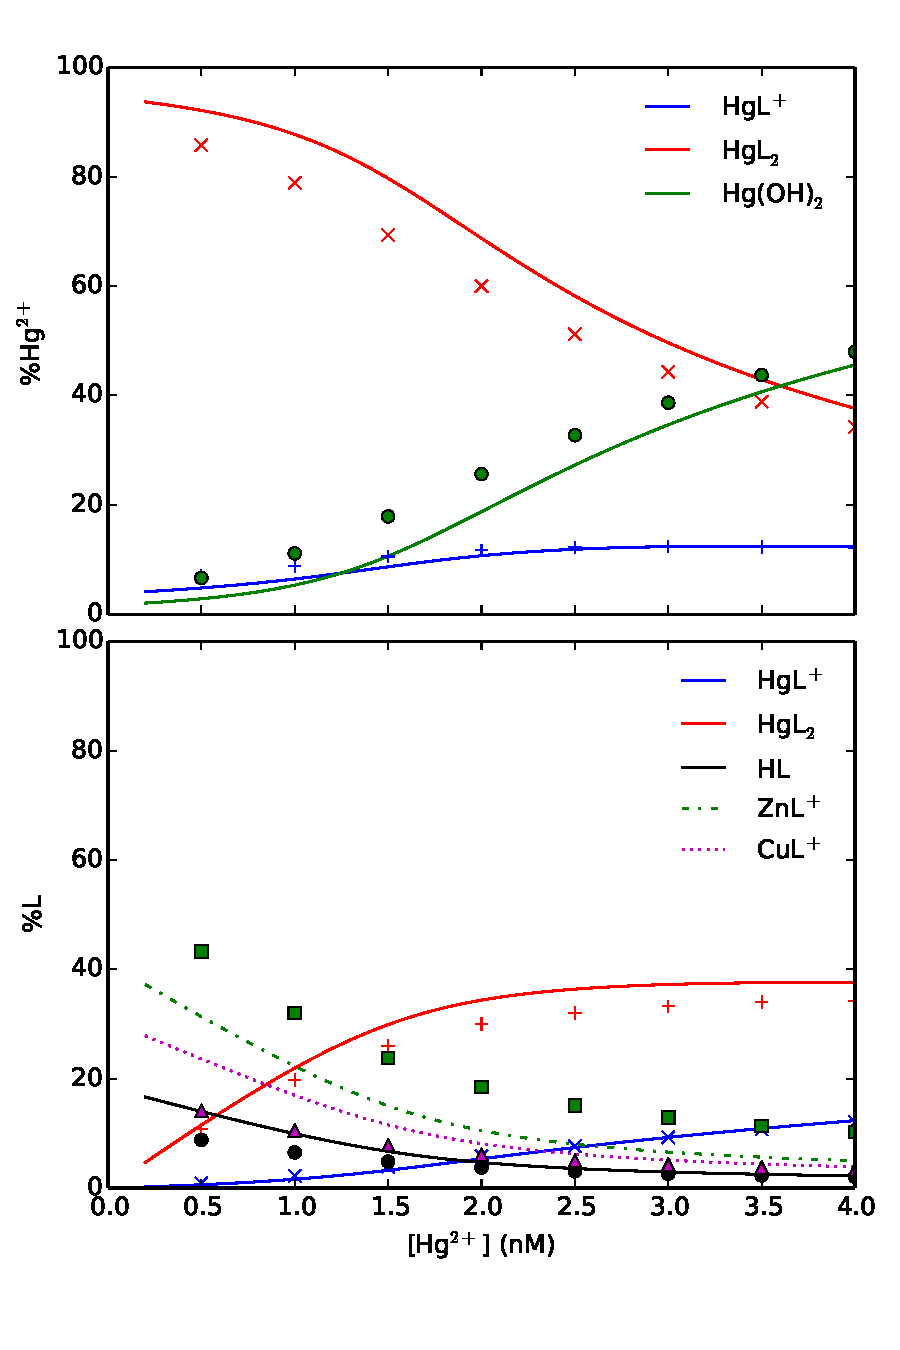
\includegraphics[width=0.5\textwidth]{../pflotran/speciation/Dong2010/ex4/ex4.pdf}
\caption{xxx}
\label{Fig4}
\end{figure}


%\newpage
\clearpage
%\cleardoublepage
%\bibliographystyle{plain}
%\bibliographystyle{plainnat}
%\bibliography{monod}

\end{document}
